\documentclass[10pt,a4paper]{scrartcl}

\usepackage[T1]{fontenc}
\usepackage[ngerman]{babel}
\usepackage[utf8]{inputenc}

\usepackage{amssymb}
\usepackage{amsmath}
\usepackage{graphicx}

\usepackage{xcolor,cancel}

\usepackage{wrapfig}

\usepackage[margin=2.5cm]{geometry}

\renewcommand{\arraystretch}{1.2}

\newif\ifincludeExamples
\includeExamplestrue % comment out to disable examples

\title{Wahrscheinlichkeitsrechnung und Statistik}
\author{Christoph H\"usler $\langle$chuesler@hsr.ch$\rangle$ } 

\DeclareMathOperator{\var}{var}
\DeclareMathOperator{\cov}{cov}

\begin{document}
\maketitle
\section{Kombinatorik}
\begin{description}
\item[Produktregel] Auswahl von $k$ aus $n$ Objekten, die einzelnen Elemente sind \emph{unabhängig} voneinander: $$n^k$$
\item[Permutation] Mögliche Anordnungen (Reihenfolge, Permutation) von $n$ Objekten $$n!$$
\item[Kombination] Auswahl von $k$ aus $n$ Objekten, wobei jedes Objekt nur einmal gewählt werden kann:
    $$\frac{n(n-1)\cdots(n-k+1)}{1 \cdot 2 \cdots k} = \frac{n!}{k!(n-k)!} = \binom{n}{k}$$
    Die erste dieser Formeln ist gut geeignet zur Umsetzung in Integer, da Divisionen immer aufgehen und Zwischenresultate ``klein'' bleiben.
\end{description}

Für kompliziertere Situationen, z.B. mit Nebenbedingungen, lässt sich oft Symmetrie ausnutzen.

\ifincludeExamples
\subsection{Erzeugende Funktion}
Schwierige kombinatorische Fragestellungen lassen sich oft in ein algebraisches oder analytisches Problem umformulieren, welches wir per Computer lösen können.

\subsubsection{Beispiel: Bildung eines Betrags aus 1 und 5 Fr. Münzen} 
\paragraph{Teilaufgabe 1} Es gibt 1 Variante, den Betrag mit 1 Fr. Münzen zu bilden.
Die erzeugende Funktion sieht wie folgt aus (geometrische Reihe): $$1 + 1x + 1x^2 + 1x^3 + 1x^4 + \dots = \frac{1}{1-x}$$ 

\paragraph{Teilaufgabe 2} Wenn der Betrag durch 5 teilbar ist, gibt es genau eine Art den Betrag mit 5 Fr. Münzen zu bilden, wenn nicht, keine.
$$1 + 0x + 0x^2 + \dots + 1x^5 + 0x^6 + \dots  = 1 + x^5 + x^{10} + x^{15} + \cdots = \frac{1}{1-x^5}$$

\paragraph{Interpretation}
Der Koeffizient $a$ von $ax^k$ sagt aus, auf wie viele Arten ein Betrag von k Fr.\ gebildet werden kann. Das Produkt der beiden Reihen kombiniert dann die 1Fr. und 5Fr. Varianten (analog erweiterbar für weitere Münzen):
$$\operatorname{taylor}\left(\frac{1}{(1-x)(1-x^5)}, 0\right) = 1 + x + x^2 + x^3 + x^4 + 2x^5 + 2x^6 + \dots + 3x^{10} + \dots$$

Äquivalent kann das Problem auch als Serie von Vektoren ausgedrückt werden, welche per Faltung (Convolution) kombiniert werden.
\fi

\section{Ereignisse und ihre Wahrscheinlichkeit}
\subsection{Ereignis}
Ein Ereignis ist immer verbunden mit einem (wiederholbaren) Experiment. Entscheidend ist der Versuchsausgang.

$$\Omega = \text{Menge der Elementar-Ereignisse} = \left\{ \text{alle möglichen Versuchsausgäng}e \right\}$$
Ein Ereignis ist eine Teilmenge von $\Omega$. Die Menge aller Ereignisse ist also die Menge aller Teilmengen von $\Omega$ (auch wenn viele davon unmöglich sind).

\ifincludeExamples
Beispiel: 7er-Würfel: $\Omega = \left\{ 1, 2, 3, 4, 5, 6, 7 \right\}$, 
2 6er-Würfel: $\Omega = \left[1, 2, 3, 4, 5, 6\right] \times \left[1, 2, 3, 4 ,5, 6\right]$\\ 
\fi

Es können auch kompliziertere Ereignisse $A \subset \Omega$ definiert werden.
\ifincludeExamples
$$G = \text{``gerade Zahl gewúrfelt''} = \{2, 4, 6\}$$
$$U = \text{``ungerade Zahl gewúrfelt''} = \{1, 3, 5, 7\}$$
$$P = \text{``Primzahl gewúrfelt''} = \{2, 3, 5, 7\}$$
\fi

\subsection{Wahrscheinlichkeit}
Wir brauchen eine ``Übersetzungstabelle'' von der Alltagssprache in die Mengensprache. 

\begin{center}
\begin{tabular}{rl}
Ereignis A eingetreten & Versuchsausgang $\omega \in A$ \\ 
Ereignis A ist unmöglich & $\forall \omega: \omega \notin A \ \Rightarrow \ A = \varnothing \ \text{(das unmögliche Ereignis)}$  \\ 
Ereignis A trifft sicher ein & $\forall \omega: \omega \in A \ \Rightarrow \ A = \Omega \ \text{(das sichere Ereignis)}$ \\ 
A und B & $A \cap B$ \\ 
A oder B & $A \cup B$ \\ 
nicht A & $\Omega \setminus A$ \\ 
wenn A dann B & $A \subset B$  \\ 
A unter der Bedingung B & $A\ |\ B$ \\
\end{tabular}
\end{center}

Die Wahrscheinlichkeit eines Ereignisses $A$ wird geschrieben als $P(A)$.

$$P(A) = \lim_{\text{\footnotesize\#Versuche} \rightarrow \infty} \frac{\text{Anzahl Eintreten von A}}{\text{Anzahl Versuche}}$$

\ifincludeExamples
Beispiel fairer (7er-)Würfel: $$P(\{7\}) = \frac{1}{7},\ P(G) = \frac{3}{7}, \ P(\varnothing) = 0, \ P(\Omega) = 1$$
\fi

Die gemessenen Werte konvergieren mit einem Fehler der Grössenordnung $\frac{1}{\sqrt{n}}$ (eine Nachkommastelle mehr entspricht $10^2$ mal mehr Experimenten).

\subsubsection{Formeln für Wahrscheinlichkeiten} 

\begin{center}
\begin{tabular}{rl}
$A \subset B$ & $P(A) \leq P(B)$ \\
$\varnothing \subset A \subset \Omega$ & $0 = P(\varnothing) \leq P(A) \leq P(\Omega) = 1$ \\
$\bar{A}$ & $P(\bar{A}) + P(A) = 1 \Rightarrow P(\bar{A}) = P(\Omega \setminus A) = 1 - P(A)$ \\
$A \cup B$ & $ P(A\cup B) = P(A) + P(B) - P(A\cap B)$ \\
A, B unabhängig & $P(A\cap B) \stackrel{!}{=} P(A)P(B)$\\[2pt]
$A\ |\ B$ & $P(A\ |\ B) = \frac{P(A\cap B)}{P(B)}$ \\[2pt]
$A$ wenn $A\ |\ B_i$ vorliegen & $ P(A) = \sum_{i=1}^n P(A\ |\ B_i) \cdot P(B_i) $
\end{tabular}
\end{center}

Intuition für diese Regeln ist die ``Flächenmessung'' (manchmal tatsächlich der Fall, z.B. Dartspiel).

\subsubsection{Satz von Bayes}
\begin{align*}
\text{Aus}\quad P(A \cap B) = P(B|A) & \cdot P(A) = P(A|B) \cdot P(B) \quad\text{folgt}\\
  P(A|B) = P(B|A) \cdot \frac{P(A)}{P(B)}\quad & \text{und} \quad P(B|A) = P(A|B) \cdot \frac{P(B)}{P(A)}
\end{align*}

\ifincludeExamples
\subsection{DNA-Test vor Gericht}
Mögliche Ereignisse:
\begin{itemize}
\item $D$ = DNA am Tatort entspricht DNA des Angeklagten
\item $T$ = Test zeigt Übereinstimmung
\end{itemize}

\begin{description} % use text for text in math environment ($ for inline resp. $$) 
\item[Anklage] $P(D|T) \text{ gross, also ist der Angeklagte der Täter}$
\item[Gericht] $P(T|D) = \text{Zuverlässigkeit des Tests}$
\item[Firma] $P(D|T) = \text{Testet, ob DNA-Test bei Übereinstimmung Ja sagt}$
\end{description}

Im Gerichtssaal: $P(D|T) = P(T|D) \cdot \frac{P(D)}{P(T)}$

Für ein wasserdichtes Alibi gilt: $P(D) = 0 \rightarrow P(D|T) = 0$ (Wasserdichtes Alibi schlägt DNA-Test).

Je grösser $P(T)$, desto kleiner $P(D|T)$, also die Wahrscheinlichkeit, dass man von diesem Test auf den Täter schliessen kann.

\subsection{HIV-Test}
Mögliche Ereignisse:
\begin{itemize}
\item $H$ = Kandidat hat Krankheit
\item $T$ = Test zeigt HIV an
\end{itemize}

Wir sind an $P(H|T)$ interessiert.

Wir `wissen':
\begin{itemize}
\item $P(H) = 0.0001$
\item $P(T|H) = 0.999$ Test zeigt HIV positiv bei einer infizierten Person an
\item $P(\bar{T}|\bar{H}) = 0.9999$ Test zeigt HIV negativ bei einer nicht infizierten Person an
\end{itemize}

\begin{align*} % & in each line will be aligned
P(H|T) &= P(T|H) \cdot \frac{P(H)}{P(T)} \quad\text{aber wir haben } P(T) \text{ nicht} \\
P(T) &= P(T|H) \cdot P(H) + P(T|\bar{H}) \cdot P(\bar{H}) \\
	 &= 0.999 \cdot 0.0001 + (1-0.9999) \cdot (1-0.0001) \\
	 &= 0.00019989 \approx 0.0002 \\
\Rightarrow P(H|T) &= 0.999 \cdot \frac{0.0001}{0.0002} \approx 0.5
\end{align*}

Umgekehrt:
$$P(\bar{H}|\bar{T}) = P(\bar{T}|\bar{H}) \cdot \frac{P(\bar{H})}{P(\bar{T})}
 = 0.9999 \cdot \frac{0.9999}{0.9998} \approx 1$$

\subsection{Karies bei Kindern und Schokoladenkonsum}
%Prüfungsaufgabe
Mögliche Ereignisse
\begin{itemize}
\item $Z$ = {schlechte Zähne}
\item $S$ = {Schoggikonsum}
\end{itemize}

Wir wissen:
$$P(Z) = 0.06 \qquad P(S|Z) = \frac{2}{3} \qquad P(S|\bar{Z}) = 0.17$$
\begin{align*}
P(Z|S) & = P(S|Z) \cdot \frac{P(Z)}{P(S)} \\
 P(S) & = P(S|Z) \cdot P(Z) + P(S|\bar{Z}) \cdot P(\bar{Z}) \\
 & = \frac{2}{3} \cdot 0.06 + 0.17 (1-0.06) \\
 & = 0.1998 \approx 20\% \\
 P(Z|S) &= \frac{2}{3} \cdot \frac{0.06}{0.2} = 20\%
\end{align*}

\subsection{Ziegen und Autos (Monty Hall-Problem)}
\begin{itemize}
\item 3 Türen: 1 Auto, 2 Ziegen
\item 1 von 3 Türen wählen
\item 2 Strategien: Bleiben, Wechseln
\end{itemize}

Ereignisse:
\begin{itemize}
\item $G = \text{Auto gewonnen}$
\item $A = \text{erste Wahl war ein Auto}$
\item $\bar{A} = \text{erste Wahl war eine Ziege}$
\end{itemize}

Finde Gewinnwahrscheinlichkeit
$$P(G) = P(G|A) \cdot P(A) + P(G|\bar{A}) \cdot P(\bar{A})$$
\begin{description}
\item[Strategie \emph{Bleiben}] $1 \cdot \frac{1}{3} + 0 \cdot \frac{2}{3} = \frac{1}{3}$
\item[Strategie \emph{Wechseln}] $0 \cdot \frac{1}{3} + 1 \cdot \frac{2}{3} = \frac{2}{3}$
\end{description}
\emph{Wechseln} ist also doppelt so gut wie \emph{Bleiben}.

\subsubsection{Strategie mit Münzwurf festgelegt}
\begin{itemize}
\item $B$: Bleibstrategie wurde gewählt
\item $W$: Wechselstrategie wurde gewählt
\end{itemize}
\begin{align*}
P(G) & = P(G|B) \cdot P(B) + P(G|W) \cdot P(W) \\
	& = \frac{1}{3}\cdot\frac{1}{2} + \frac{2}{3}\cdot\frac{1}{2} = \frac{1}{2}
\end{align*}
Optimale Strategie: Immer wechseln.

\subsection{Das Erfolgsgeheimnis von Google}
\begin{description}
\item[Problem] Vorkommen von Wörtern sagt nichts (mehr) über Relevanz aus.
\item[Idee von Google] Relevanz aus Internet $\rightarrow$ Pagerank. Finde Seite mit höchster Relevanz aus Linkstruktur.
\end{description}

\begin{figure}
    \centering
    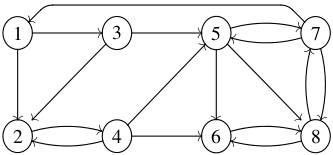
\includegraphics[width=0.4\textwidth]{images/google-internet.png}
    \caption{Beispiel-Internet mit 8 Knoten}
    \label{fig:awesome_image}
\end{figure}

Ereignisse:
\begin{itemize}
\item $S_{i}$ = Surfer liest Seite $i$ ($P(S_i)$ misst Beliebtheit der Seite $S_i$)
\item $S_{j}'$ = Surfer liest Seite $j$ nachdem er geklickt hat.
\end{itemize}

Aus dem Satz der Totalen Wahrscheinlichtkeit folgt
$$P(S_j') = \sum_{i=1}^N P(S_j' | S_i) \cdot P(S_i)$$

Da die Anzahl Besucher pro Webseite vor und nach einem Klick ungefähr gleich bleibt können wir $P(S_j') = P(S_j)$ gleichsetzen. Dies ergibt ein Gleichungssystem (eine Gleichung pro Webseite).

$$H = 
\begin{matrix}
  S_1 & S_2 & S_3 & S_4 & S_5 & S_6 & S_7 & S_8 &  \\
  0 & 0 & 0 & 0 & 0 & 0 & \frac{1}{3} & 0 & S_1' \\
  \frac{1}{2} & 0 & \frac{1}{2} & \frac{1}{3} & 0 & 0 & 0 & 0 & S_2' \\
  \frac{1}{2} & 0 & 0 & 0 & 0 & 0 & 0 & 0 & S_3' \\
  0 & 1 & 0 & 0 & 0 & 0 & 0 & 0 & S_4' \\
  0 & 0 & \frac{1}{2} & \frac{1}{3} & 0 & 0 & \frac{1}{3} & 0 & S_5' \\
  0 & 0 & 0 & \frac{1}{3} & \frac{1}{2} & 0 & 0 & \frac{1}{2} & S_6' \\
  0 & 0 & 0 & 0 & \frac{1}{2} & 0 & 0 & \frac{1}{2} & S_7' \\
  0 & 0 & 0 & 0 & 0 & 1 & \frac{1}{3} & 0 & S_8' 
\end{matrix}$$


\begin{align*}
P(S_{j}') &= \sum\limits{i=1}^N P(S_{j}'|S_{i}) \cdot P(S_{i}) \\
P(S_{j}'|S_{i}) &= \text{Zeile von } H \\
\text{mit } p = \begin{pmatrix}
\dots \\
P(S_{j}) \\
\dots
\end{pmatrix},\quad p' &= Hp
\end{align*}

Mit der Zeit stabilisieren sich die Wahrscheinlichkeiten $P(S_i)$ und $p$ konvergiert zum Eigenvektor mit Eigenwert 1 von $H$.

\subsubsection{Berechnung des Eigenwertes}
$H$ ist eine sehr spezielle Matrix. Alle Spalten summieren zu $1$ auf, und alle anderen Eigenwerte sind kleiner als $1$.

\begin{align*}
p &= a_pp + a_1v_1 + a_2v_2 + \dots \\
H^np &= a_pp + a_1\lambda_1^nv_1 + a_2\lambda_2^nv_2 + \dots \\
\Rightarrow H^np &=a_pp
\end{align*}

Da die $\lambda_i$ alle kleiner als 1 sind verschwinden diese Terme mit grösseren $n$, und übrig bleibt $p$

\subsubsection{Freier Wille}
F: Surfer setzt freien Wille ein. $P(F) = 1 - \alpha$ (Konfigurationsparameter).

\begin{align*}
P(S_{j}') & = P(S_{j}'|F)\cdot P(F) + P(S_{j}'|\bar{F})\cdot P(\bar{F}) \\
\Rightarrow p & = \frac{1}{N}\cdot (1-\alpha) +  \alpha Hp
\end{align*}

G ist die Google-Matrix, A ist eine Matrix voller Einsen.
$$
p = Gp = \alpha Hp + (1-\alpha)\frac{1}{N}Ap \rightarrow G = \alpha H + (1-\alpha)\frac{1}{N}A 
$$
\fi

\section{Zufallsvariablen, Erwartungswert, Varianz}

\subsection{Zufallsvariablen}

Ereignisse treffen ein oder nicht. Wir wollen Versuchsausgängen aber einen Wert zuweisen können.
Beim Würfeln haben wir die unterschiedlichen Bilder auf den Würfel-Seiten als Wert interpretiert, d.h. wir haben implizit eine Funktion 
$$X: \Omega \rightarrow \mathbb{R}\ :\ \omega \rightarrow X(\omega)$$

$X$ ist eine Zufallsvariable (ZV). Diese Zufallsvariable definiert nun neue Ereignisse:
\begin{align*}
\{ X = x \} \quad& P(X = x) \\
\{ X \le a \} \quad& P(X\le a) \\
\{ X > a \} \quad& P(X > a)
\end{align*}

\subsection{Erwartungswert}
$X$ ist eine Zufallsvariable.

$$E(X) = \sum_{\text{Werte}} \text{Wert} \cdot \text{Wahrscheinlichkeit} = \sum_{i=1}^n x_i \cdot P(X = x_i) $$

\ifincludeExamples
\begin{center}
\begin{tabular}{c | c | c} 
Werte & Wahrscheinlichkeit \\ \hline
1 & $\frac{1}{6}$ & $1 \cdot \frac{1}{6}$ \\
2 & $\frac{1}{6}$ & $2 \cdot \frac{1}{6}$ \\
3 & $\frac{1}{6}$ & $3 \cdot \frac{1}{6}$ \\
4 & $\frac{1}{6}$ & $4 \cdot \frac{1}{6}$ \\
5 & $\frac{1}{6}$ & $5 \cdot \frac{1}{6}$ \\
6 & $\frac{1}{6}$ & $6 \cdot \frac{1}{6}$ \\ \cline{3-3}
\multicolumn{2}{c|}{} & $\frac{21}{6} = 3.5$  
\end{tabular}
\end{center} 

Intuition: Erwartungswert $E(X)$ verhält sich wie ein Integral $\int f(x) dx$.
\fi

\subsubsection{Rechenregeln für Erwartungswerte $E(\ .\ )$}

$E(\ .\ )$ ist eine lineare Funktion.
\begin{align*}
\text{Add. Linearität: } & E(X+Y) = E(X) + E(Y) \\
\text{Mult. Linearität: } & E(\lambda X) = \sum_{i=1}^n \lambda x_i P(X = x_i) = \lambda \sum_{i=1}^n x_i P(X = x_i) \\
X \text{ und } Y \text{ unabhängig } &\Longleftrightarrow \forall x,y: \{ X = x \} \text{ und } \{Y = y\} \implies E(XY) = E(X)E(Y)
\end{align*}

\subsection{Varianz}
Varianz ist die Abweichung nach ``links'' und ``rechts''. Intuitiv: $X - E(X)$. Aber:
$$ E(X - E(X)) = E(X) - E(E(X)) = E(X) - E(X) = 0 $$
Die negativen Vorzeichen stellen ein Problem dar. Da Beträge aus analytischer Sicht suboptimal sind (Nullpunkt) ist die Lösung die Quadratfunktion.

\begin{align*}
 \text{Varianz } \var(X) &= E((X - E(X))^2)  \\
 \text{Einfachere Formel: } \var(X) &= E(X^2 - 2XE(X) + E(X)^2) \\
& = E(X^2) - 2E(X)E(X) + E(X)^2 \\
& = E(X^2) - E(X)^2
\end{align*}

\ifincludeExamples
\subsubsection{Beispiel}
\begin{center}
\begin{tabular}{c | c | c | c | c}
X & P & $X^2$     & $X \cdot P(X)$ & $X^2 \cdot P(X)$ \\ \hline
1 & $\frac{1}{6}$ & 1  & $\frac{1}{6}$ & $\frac{1}{6}$ \\
2 & $\frac{1}{6}$ & 4  & $\frac{2}{6}$ & $\frac{4}{6}$ \\
3 & $\frac{1}{6}$ & 9  & $\frac{3}{6}$ & $\frac{9}{6}$ \\
4 & $\frac{1}{6}$ & 16 & $\frac{4}{6}$ & $\frac{16}{6}$ \\
5 & $\frac{1}{6}$ & 25 & $\frac{5}{6}$ & $\frac{25}{6}$ \\
6 & $\frac{1}{6}$ & 36 & $\frac{6}{6}$ & $\frac{36}{6}$ 
\end{tabular}
\end{center}

\begin{align*}
E(X) &= \frac{21}{6} = \frac{7}{2}, \quad E(X^2) = \frac{91}{6} \\
\var(X) & = E(X^2) - E(X)^2 = \frac{91}{6} - \frac{49}{4} = \frac{35}{12} \\
\sqrt{\var(X)} &\approx 1.707 \\
\end{align*}
\fi

\subsubsection{Rechenregeln für Varianz}
\begin{align*}
\var(\lambda X) & = E((\lambda X)^2) - E(\lambda X)^2  = \lambda^2 E(X^2) - \lambda^2E(X)^2 \\
               & = \lambda^2 \var(X) \\
\var(X+Y)       & = E((X+Y)^2) - E(X+Y)^2 \\
               & = E(X^2) + 2E(XY) + E(Y^2) - E(X^2) - 2E(X)E(Y) - E(Y^2) \\
               & = \var(X) + \var(Y) + 2(\underbrace{E(XY) - E(X)E(Y)}_{\cov(X, Y)}) 
\end{align*}

$\cov$ ist die Kovarianz, welche ist 0 wenn $X$ und $Y$ unabhängig sind.

\subsection{Genauigkeit des Mittelwertes}
$X$: Zufallsvariable, $\mu = E(X)$, $\,\varepsilon$: erwünschte Genauigkeit. \\
Gesucht: $ P(|X - \mu| > \,\varepsilon) $
 
\begin{itemize}
\item $\,\varepsilon \text{ klein } \Rightarrow P (|X-\mu| > \,\varepsilon) \text{ gross}$.
\item $\var(X) \text{ grösser } \Rightarrow P (|X-\mu| > \,\varepsilon) \text{ grösser}$.
\end{itemize}

\subsubsection{Satz von Tschebyscheff}
 $$P (|X-\mu| > \,\varepsilon) \le \frac{\var(X)}{\,\varepsilon^2}$$
\ifincludeExamples
\subsubsection{Beweis}
\begin{align*}
\text{Ereignis } A &= \{ |X-\mu| > \,\varepsilon \} \\
\text{besondere ZV: } \chi_A & = \begin{cases}1 & \quad A \text{ eingetreten} \\ 
                                              0 & \quad \text{sonst}
                                 \end{cases} & \text{logischerweise: } \chi^2 = \chi\\
E(\chi_A) & = 0\cdot P(\chi_A = 0) + 1\cdot P(\chi_A = 1) = P(A) \\
\varepsilon &\le |X - \mu| & \text{gilt falls } A \text{ eingetreten} \\
\varepsilon \chi_A &\le |X-\mu| & ()^2 \text{ statt Betrag} \\
\varepsilon^2\chi_A^{\cancel{2}} &\le (X-\mu)^2 & |\ E(\ .\ ) \\
\varepsilon^2P(A) = \,\varepsilon^2E(\chi_A)&\le E((X-E(X))^2) = \var(X) \\
\varepsilon^2P(|X-\mu|>\,\varepsilon) & \le \var(X)
\end{align*}
\fi

\subsubsection{Genauigkeit erhöhen}
Viele Messungen $X_1, X_2, \dots, X_n$. $ \text{Mittelwert } M_n = \frac{X_1+ X_2+ \dots + X_n}{n}$ wird \emph{genauer} mit mehr Messungen.

\begin{align*}
E(M_n) & = E\left( \frac{X_1+ X_2+ \dots + X_n}{n}\right)  \\
& = \frac{E(X_1) + E(X_2) + \dots + E(X_n)}{n} \\
& = E(X) \\
\var(M_n) &= var\left(\frac{X_1+ X_2+ \dots + X_n}{n}\right) \\
&\stackrel{\text{falls }X_i\text{ unabhängig}}{=} \frac{\var(X_1)+ \var(X_2)+ \dots + \var(X_n)}{n^2} \\ % FIXME text should be above =
& = \frac{n\cdot \var(X)}{n^2} \\
& = \frac{\var(X)}{n}
\end{align*}
Die Varianz wird also kleiner bei mehr \emph{unabhängigen} Messungen.

$$ P(|M_n - \mu| > \,\varepsilon) \le \frac{\var(M_n)}{\,\varepsilon^2} = \frac{\var(X)}{n\,\varepsilon^2} $$
Erwartungswert und Varianz lassen sich nun wie folgt ausdrücken:
\begin{align*}
E(X) & = \lim_{n\to\infty} \frac{1}{n} \sum_{i=1}^n x_i \\
\var(X) & = \frac{1}{n} \sum_{i=1}^n x_i^2 - \left(\frac{1}{n} \sum_{i=1}^n x_i\right)^2
\end{align*}
Je mehr Messungen vorhanden sind, desto weniger wahrscheinlich ist eine Abweichung grösser als $\,\varepsilon$ (\emph{Gesetz der grossen Zahlen}).

Falls $P(|M_n - \mu| > \,\varepsilon) \le p$ sein soll:
\begin{align*}
  p & \le \frac{\var(X)}{n\,\varepsilon^2} \quad\Rightarrow\quad
  n \le \frac{\var(X)}{p\,\varepsilon^2} \\
  \text{worst case: } n &= \frac{\var(X)}{p\,\varepsilon^2} \quad {d.h.}\quad n \sim \frac{1}{\,\varepsilon^2}
\end{align*}

\subsection{Wie genau ist die Häufigkeit als Mass für die Wahrscheinlichkeit?}
Ereignis $A$ mit Wahrscheinlichkeit $P(A)$.

\begin{align*}
  h_n = \frac{\text{Anzahl eingetreten}}{n} & & P(|h_n - P(A)| > \,\varepsilon) =\text{ ?} \\% P(A) = E(\chi_A), \chi_A = X
h_n = \frac{X_1 + X_2 + \dots + X_n}{n} = M_n& & P(|M_n - \mu| > \,\varepsilon) \le \frac{\var(\chi_A)}{n\,\varepsilon^2} 
\end{align*}

\begin{align*}
\var(\chi_A) & = E(\chi_A^{\cancel{2}}) - E(\chi_A)^2 \\
& = P(A) - P(A)^2 \\
& = P(A) (1 - P(A)) \\
P(|h_n - P(A)| > \,\varepsilon) & \le \frac{P(A)(1-P(A))}{n\,\varepsilon^2} \le \frac{1}{4n\,\varepsilon^2} \qquad(\text{da } x(1-x) \le \frac{1}{4})
\end{align*}

\subsection{Anwendung: Lineare Regression}
Zwei Zufallsvariablen $X$, $Y$, mit $Y\approx aX+b$. Das Ziel ist, aus Messungen $a$ und $b$ zu ermitteln.

\ifincludeExamples
\paragraph{Beispiel: Wie lange muss ein Verzögerungselement sein?}

\begin{itemize}
\item Konstante Abbrand-Geschwindigkeit, d.h. linearer Zusammenhang zwischen Länge und Brenndauer. $$L = aT + b$$
\end{itemize}

\begin{center}
\begin{tabular}{c|c|c}
& T, & L \\ \hline
1 & $t_1$ & $l_1$ \\
\dots & \dots  & \dots \\
5 & $t_5$ & $l_5$
\end{tabular}
\end{center}

% TODO: Graph t/l mit Punkten nicht ganz auf gerade

Gesucht ist nun $L = aT + b + Fehler$ mit möglichst kleinem Fehler.
\fi

\paragraph{Problem}
X, Y sind Zufallsvariablen, finde $a$, $b$ so, dass $Y-aX-b$ minimal.
\paragraph{Gesucht}
\begin{enumerate}
\item Im Mittel kein Fehler: $0 = E(Y - aX-b) = E(Y) - aE(X) - b$
\item Möglichst kleine Varianz: $var(Y-aX-b)$ möglichst klein
\end{enumerate}

Das ist ein Optimierungsproblem. Idee: Ableiten.

\begin{align*}
  \var(Y - aX - b) &= E((Y-aX-b)^2) - E(Y-aX-b)^2 \\ 
                   &= E(Y^2) + a^2E(X^2) + \cancel{b^2} - 2aE(XY) - \cancel{2bE(Y)} + \cancel{2abE(X)} - \\
                   &  \quad \left(E(Y)^2 + a^2E(X)^2 + \cancel{b^2} - 2aE(X)E(Y) - \cancel{2bE(Y)} + \cancel{2abE(X)}\right) \\
                   &=  \var(Y) + a^2\var(Y) - 2a\cov(X, Y) = Q\\[0.2cm]
  \frac{\partial Q}{\partial a} &= 2a\var(Y) - 2\cov(X, Y) = 0 \\
                   a &= \frac{\cov(X, Y)}{\var(X)} \\
                   b &= E(Y) - aE(X)
\end{align*}

\end{document}
